\chapter{Surfing Mechanics}

%%%%%%%%%%%%%%%%%%%%%%
\section{Introduction}

Avoid being a kook by reading the rules of surfing \cite{borte2013kook}.

% use the [] inside the caption for short titles that go into the List of Figures at the beginning
\begin{figure*}[hbt!]
  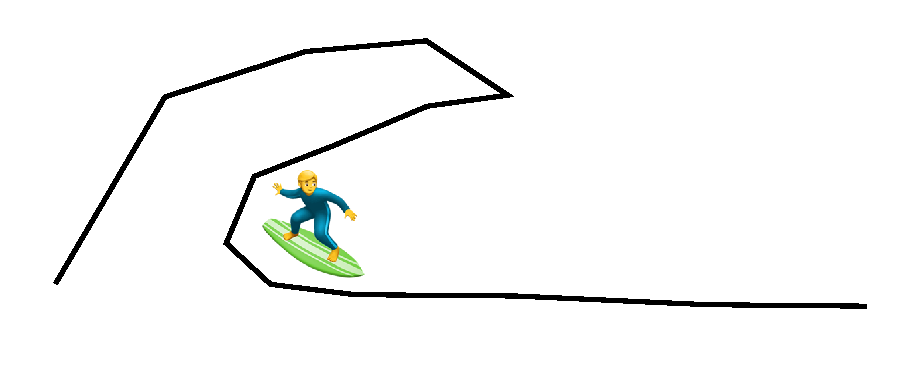
\includegraphics{figures/chap3/surf.pdf}
  \caption[Shreddie Getting Barreled]{Shreddie McShredface showing everyone how to get barreled.}
  \label{fig:TPM}
\end{figure*}

\lipsum[2]

\begin{table}[hbt!]\centering
\captionsetup{justification=centering}
\captionsetup{width=.6\textwidth}
\captionsetup{skip=2pt}
\caption{Wave Statistics}
\renewcommand{\arraystretch}{1.5}
\begin{threeparttable}
\begin{tabular}{cccc}\toprule
  {Wave Height} & {Awesomeness\tnote{a}} \\ \midrule
    1-2 & 4\\
    2-4 & 8\\
    4-6 & 10\\
    6-8 & 8\\
    8-10 & 6\tnote{b}\\ \bottomrule
\end{tabular}
\begin{tablenotes}
\item[a] \footnotesize Awesomeness is on a 1-10 scale, 1 being the min and 10 being the max awesomeness
\item[b] \footnotesize This would be higher if you weren't afraid for your life
\end{tablenotes}
\end{threeparttable}
\end{table}
